\section{Investigacion}
\subsection{Introducci\'on}

Se nos asign\'o la lectura y an\'alisis del paper \emph{Job Scheduling for Multi-User MapReduce Clusters}, de la universidad de ciencias de computaci\'on de California en Berkeley. Como su nombre indica, la raz\'on principal del paper es la identificac\'ion y b\'usqueda de soluciones a diversos problemas que poseen los schedulers de clusters Map-Reduce al ser compartidos por varios usuarios.

\vspace{2mm}

Map-Reduce, y su implementaci\'on open source \emph{Hadoop}, fueron optimizados originalmente para tareas largas de tipo \emph{batch}. Sin embargo, \'ultimamente ha emergido un nuevo caso de uso, compartir un cluster Map-Reduce entre diversos usuarios, quienes corren tareas \emph{batch} y adem\'as \emph{querys} cortas interactivas, sobre un conjunto com\'un de datos.

\vspace{2mm}

Compartir un cluster Map-Reduce posee diversas ventajas, permite realizar \emph{statistical multiplexing}, lo cual tiene un costo mucho menor a la construcci\'on de clusters individuales, evita la r\'eplica de datos, mejora la \emph{consolidaci\'on} de los datos, lo cual maneja eficientemente \emph{querys} ad-hoc entre conjuntos disjuntos de datos  y por \'ultimo, conlleva a brindar acceso a diversos usuarios a un conjunto de datos muy grande. Sin embargo, los algoritmos tradicionales de scheduling pueden tener muy mala perfomance con Map-Reduce, debido a la necesidad de tener \textbf{localidad} de datos, y a la \textbf{dependencia} entre las tareas Map y Reduce.

\subsection{Entorno y motivaci\'on de la investigaci\'on}

El trabajo de los autores fue motivado en el an\'alisis de la carga de trabajo Map-Reduce de la conocida red social \emph{Facebook}. \'Esta posee un cluster de datos implementado en \emph{Hadoop}, el cual recibe \emph{logs} de eventos del sitio web cada hora, donde son usados para una gran variedad de aplicaciones, como el an\'alisis de patrones de uso para la mejora del disenio del sitio, detecci\'on de spam, \emph{data mining} y optimizaci\'on. 	A medida que \emph{Facebook} constru\'ia su servidor de datos, encontr\'o muy atractiva la consolidaci\'on de lo datos que provee un cluster compartido. Por ejemplo, un ingeniero trabajando en detecci\'on de \emph{spam} podr\'ia buscar patrones en fuentes de dato arbitrarias, como listas de amigos o clicks de publicidad, para identificar \emph{spammers}

\vspace{2mm}

El servidor corre en 600 equipos, almacena 500 TB de datos comprimidos, los cuales crecen a raz\'on de 2 TB diarios. Se corren tareas peri\'odicas de producci\'on, y adem\'as tareas experimentales, desde c\'omputos de aprendizaje autom\'atico de varias horas, hasta \emph{querys} ad-hoc de un par de minutos, ingresadas a trav\'es de una interfaz \emph{SQL} llamada \emph{Hive}. El sistema corre aproximadamente 32000 tareas Map-Reduce diarias, y es usado por m\'as de 50 ingenieros de \emph{Facebook}.

\subsection{Identificaci\'on del problema}

Lamentablemente, ni bien varios grupos de trabajo de \emph{Facebook} comenzaron a utilizar \emph{Hadoop}, comenzaron a sufrir los tiempos de respuesta de las tareas, debido al \textbf{Scheduler FIFO} de \emph{Hadoop}. Esto era inaceptable para las tareas de producci\'on, e hizo imposible la ejecuci\'on de \emph{querys} interactivas, reduciendo enormemente la utilidad del sistema. Diversos grupos de \emph{Facebook} consideraron implementar clusters privados para sus tareas pero esto era demasiado costoso para ser justificado. 

\vspace{2mm}

Aunque los autores hayan motivado su trabajo con el caso \emph{Facebook}, los problemas que esto conlleva no est\'an restringidos bajo ning\'un punto de vista a servidores de datos. Diversos contactos en otros sitios web de importancia que usan \emph{Hadoop} les confimaron que la mayor queja entre los usuarios de los clusters son las largas colas de espera.

\vspace{2mm}

La mayori\'a de los problemas de Map-Reduce scheduling, a diferencia de shceduling de cluster tradicionales, son ocasionados por dos caracter\'isticas intr\'insecas y muy importantes de Map-Reduce:

\begin{enumerate}

\item \textbf{Necesidad de localidad de los datos}: Por ejemplo, almacenar las tareas en nodos que contienen sus datos de entrada. La localidad es crucial en la performance ya que el ancho de banda de una red de un cluster es mucho menor al ancho de banda agregado de los discos de los equipos.

La performance decrece significativamente en algunos schedulers tradicionales que asignan a cada usuario un conjunto fijo de equipos, como \emph{Torque}, ya que en \emph{Hadoop}, los archivos son distribu\'idos entre todos los nodos. Incluso con un scheduler granularmente justo, se encontr\'o que tareas cortas y concurrenes sufr\'ian problemas de localidad.

\item \textbf{Dependencia de datos:}. Las tareas de tipo Reduce no pueden terminar hasta que hayan terminado todas las tareas de tipo Map. Esta dependencia no se encuentra en modelos tradicionales de scheduleling de clusters, lo que conlleva a \emph{starvation} y subutilizac\'on de los recursos: una tarea pesada que adquiera \emph{slots} de Reduce en varios equipos no los liberar\'a hasta que se hayan finalizado todas las tareas, lo cual subutiliza esos \emph{slot} y genera \emph{starvation} hacia las otras tareas.

La dependencia de los datos conlleva a que los resultados intermedios producidos por el Map no pueden ser borrados hata que finalice toda el trabajo, consumiendo mucho espacio en disco. Adem\'as conlleva a din\'amicas no presentes en otras configuraciones: una asignaci\'on justa de las tareas en Map-Reduce puede hacer que la ejecuci\'on de tareas \emph{batch} tarde m\'as que con un simple algorito FIFO.

\end{enumerate}

\subsection{Scheduler FIFO de Hadoop y HOD}

La implementaci\'on de Map-Reduce de \emph{Hadoop} se parece a la de \emph{Google}. \emph{Hadoop} se ejecuta sobere un sistema de archivos distribuido, \emph{HDFS}, que almacena tres r\'eplicas de cada bloque. Los usuarios ingresan \textbf{trabajos}, que consisten de una tarea Map y una Reduce. \emph{Hadoop} divide los trabajos en m\'ultiples \textbf{tareas}. En primer lugar, las tareas Map procesan cada bloque de entrada, producen resultados intermedios, que son pares \textbf{clave-valor} y los almacenan en disco. Luego, las tareas Reduce toman estos resultados asociados a cada clave y corren la funci\'on reductora del usuario. Esto produce la salida del trabajo.

\vspace{2mm}

El scheduling de trabajos de \emph{Hadoop} es realizado por un \textbf{nodo maestro}, quien distribuye carga entre \textbf{nodos esclavo}. Las tareas son asignadas en respuesta a seniales de status enviadas por los esclavos cada par de segundos. Cada esclavo posee un n\'umero de \textbf{map slots} y \textbf{reduce slots} para sus tareas. Dado que las tareas de \emph{Hadoop} son \emph{single-thread}, hay un slot por n\'ucleo. Una de las principales ventajas de este modelo es su sencilla gesti\'on de asignaci\'on de memoria y CPU.

\subsubsection{HOD y problemas asociados}

El scheduler base de \emph{Hadoop} ejecuta los trabajos en orden \textbf{FIFO}, usando cinco niveles de prioridad. Cuando un slot de tarea se libera, el scheduler recorre los trabajos en orden de prioridad hasta encontrar uno con una tarea del tipo requerido y suficiente memoria. Para optimizar la localidad, elige la tarea que tenga sus datos en el nodo m\'as cercano al esclavo.

\vspace{2mm}

La desventaja de usar scheduling FIFO es el pobre tiempo de respuesta para los trabajos cortos en presencia de trabajos largos. La primera soluci\'on al problema fue \emph{Hadoop On Demand (HOD)}, que dispone clusters Map-Reduce privados sobre un gran cluster f\'isico usando \emph{Torque}. \emph{HOD} permite a los usuarios compartir un sistema de archivos, corriendo todos los nodos, y al mismo tiempo poseer un cluster Map-Reduce privado en sus nodos reservados. Sin embargo, \emph{HOD} posee dos problemas, anteriormente nombrados:

\begin{enumerate}

\item \textbf{Localidad pobre}: Cada cluster privado corre en un set fijo de nodos reservados, pero los archivos en \emph{HDFS} son divididos entre todos los nodos. Como resultado, algunas funciones map deben leer datos por toda la red, enlenteciendo el tiempo de respuesta y el throughput. 

\item \textbf{Subutilizaci\'on}: Dado el tamanio fijo de cada cluster privado, algunos de sus nodos pueden no utilizarse. Dado que los trabajos en \emph{Hadoop} son el\'asticos, puede cambiar su cantidad de nodos en uso, y estos nodos no utilizados podr\'ian acelerar otros trabajos. 

\end{enumerate}


\subsection{Soluci\'on propuesta: FAIR scheduler}

Los autores desarrollaron el scheduler \textbf{FAIR}, como ua soluci\'on a los problemas de \emph{HOD}. Sus objetivos principales son asegurar el \textbf{aislamiento} (dar a cada trabajo la ilusi\'on de un cluster privado), y la capacidad de redistribuir los recursos no usados de un trabajo a otros, o \textbf{statistical multiplexing}.

\vspace{2mm}

FAIR posee dos niveles de jerarqu\'ia. En el nivel superior, FAIR asigna slots de tarea en \textbf{pools}, en el segundo nivel, cada pool
asigna sus slots entre m\'ultiples trabajos. FAIR usa una versi\'on de \emph{min-max fairness} para la asignaci\'on de slots entre pools. Se define una cantidad m\'inima de slots para cada pool, y el scheduler se asegura de que en todo momento, cada pool tenga al menos esta cantidad de slots, y la suma de estas cantidades no supere los slots m\'aximos soportados por el sistema.

\vspace{2mm}

En la pr\'actica, se crea una pool por usuario y pools especiales para trabajos de producci\'on. ESto asegura para cada usuario una performance al menos id\'entica a la que tendr\'ian en un cluster \emph{Hadoop} de tamanio igual a su cantidad m\'inima, pero gracias al \emph{statistical multiplexing}, a menudo mayor. FAIR usa el mismo algoritmo para asignar slots entre los trabajos de cada pool.

\vspace{2mm}

\begin{center}
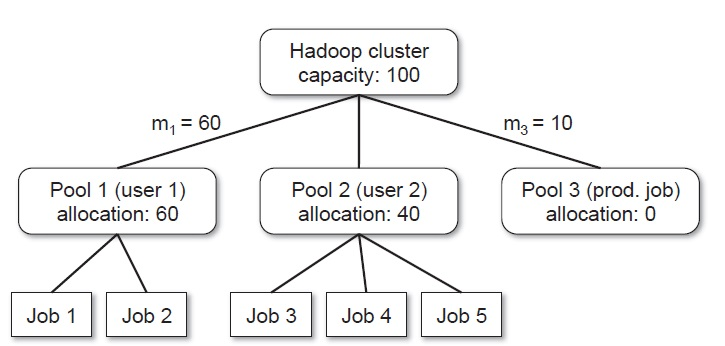
\includegraphics[scale=0.8]{pools.jpg}
\end{center}
 \textit{Diagrama de asignaci\'on de slots de FAIR'}.

\vspace{2mm}

Dado el objetivo de FAIR de asignar la totalidad de recursos de un cluster entre las pools que tienen trabajos, la principal pregunta es c\'omo reasignar slots cuando la demanda fluct\'ua. FAIR utiliza una estrategia mixta entre esperar que terminen tareas y \emph{matar} tareas, o finalizarlas forzadamente. Matar tareas no tiene consecuencias graves en \emph{Hadoop}, simplemente se considera que nunca comenzaron.

\vspace{2mm}

Cuando un trabajo comienza, FAIR comienza a asignarle slots a medida que finalizan otros trabajos. Teniendo en cuenta que las tareas Map-Reduce son generalmente cortas, un trabajo alcanza su cantidad minima de slots r\'apidamente, comparable a la velocidad de un cluster privado.
En caso de haber trabajos con tareas largas, FAIR usa dos \textbf{timeouts} para cada trabajo. Uno para garantizar que pasado el tiempo el trabajo haya conseguido su cantidad minima de slots (en caso de que no, FAIR mata tareas de otras pools y reasigna slots al trabajo), el segundo para garantizar que pasado m\'as tiempo obtenga la cantidad \textbf{justa} de slots (caso contrario, mata m\'as tareas).

\vspace{2mm}

Las tareas a matar pertenecen a trabajos sobrecargados, y se buscan las m\'as recientemente empezadas, de forma de minimizar el tiempo de c\'omputo perdido, siempre y cuando no se lleve a la cantidad de slots de un trabajo a menos de su m\'inimo.

\subsection{Problemas asociados a FAIR y sus soluciones}

Los autores analizaron y abordaron los problemas cl\'asicos que todos los schedulers presentan con Map-Reduce y \emph{Hadoop}: localidad y dependencia.

\subsubsection{Localidad de datos}

El primer problema de localidad que notaron los autores fue en los trabajos cortos. Ellos nombran al comportamiento causante de esto \emph{head-of-line scheduling}. En cada momento, hay un trabajo que debe recibir el pr\'oximo slot seg\'un el scheduler: el trabajo con m\'as slots de diferencia por debajo que la cantidad justa (el \emph{head-of-line}). Cualquier nodo esclavo que pida una tarea recibe una de este trabajo. Sin embargo, si este trabajo es pequenio, hay muy pocas posibilidades de que sus bloques de entrada est\'en disponibles en el esclavo. Este problema estaba presente en todos los schedulers de \emph{Hadoop} en ese momento.

\vspace{2mm}

El problema presentado deriva de la falta de elecci\'on del scheduler, seguir un orden de asignaci\'on estricto fuerza que se seleccione un trabajo sin datos locales. La soluci\'on de los autores a este problema tiene por nombre \textbf{Delayed scheduling}. Cuando un nodo solicita una tarea, si el trabajo al principio de la fila no posee una tarea local, se saltea y se busca en los siguientes trabajos. Sin embargo, si un trabajo fue demasiado salteado, se le permite lanzar tareas no locales para prevenir \emph{starvation}.

\subsection{Evaluac\'on}

\subsection{Discusi\'on}
